\documentclass[conference]{IEEEtran}
\IEEEoverridecommandlockouts

\usepackage[utf8]{inputenc}
\usepackage[T1]{fontenc}
\usepackage{cite}
\usepackage{amsmath,amssymb,amsfonts}
\usepackage{graphicx}
\usepackage{textcomp}
\usepackage{xcolor}
\usepackage{booktabs}
\usepackage{array}
\usepackage{multirow}
\usepackage{siunitx}
\usepackage{tikz}
\usetikzlibrary{positioning,arrows.meta,fit,calc}
\usepackage{pgfplots}
\pgfplotsset{compat=1.18}
\usepackage{pgfplots}
\pgfplotsset{compat=1.18}
\usepackage{pgfplots}
\pgfplotsset{compat=1.18}
\usepackage[hidelinks]{hyperref}

\sisetup{detect-weight=true,detect-family=true}
\newcommand{\ddimcrps}{1.222}
% IEEEtran inserts an empty row before every author block after the first one it has seen; the
% nested two-by-two author layout needs each block to start fresh so that the four blocks align.
\makeatletter
\newcommand{\authorblockreset}{\global\@IEEEprevauthorblockincolfalse}
% Inside the nested layout, IEEEtran's spacer row before each affiliation renders as a full blank line;
% replace it with a small fixed gap between an author's name and affiliation.
\let\origIEEEauthorblockA\IEEEauthorblockA
\renewcommand{\IEEEauthorblockA}{\noalign{\vskip 0.6ex\global\@IEEEprevauthorblockincolfalse}\origIEEEauthorblockA}
% keep the first affiliation line in the same font as the lines after it
\def\@IEEEauthorblockAstyle{\normalfont}
\makeatother

\begin{document}
% IEEE reference rule: more than six authors are shortened to the first author et al. (control entry in refs.bib)
\bstctlcite{IEEEexample:BSTcontrol}

% Fix the reference numbering: [1]--[5] are PV-MM-Diffusion, SKIPP'D, PARA-PV, SFT and SkyEvo; the rest follow
% the order of refs.bib. IEEEtran numbers entries in order of first citation.
\nocite{huang2026pvmm,nie2023skippd,fan2026parapv,jiang2026sft,ruan2026skyevo,
  antonanzas2016review,vandermeer2018review,sun2019sunset,nie2024skygpt,paletta2021benchmarking,
  paletta2023advances,holmgren2018pvlib,ho2020ddpm,song2021ddim,ho2022video,ruan2023mmdiffusion,
  rasul2021timegrad,tashiro2021csdi,gao2023prediff,leinonen2023ldcast,ronneberger2015unet,
  vaswani2017attention,simonyan2015vgg,kingma2015adam,lu2022dpmsolverpp,lauret2019verification,lee2018savp}

\title{Fast Sampling for Joint Sky-Image and PV Diffusion Forecasting: A 15-Step DDIM Evaluation}

\author{
\begin{tabular}{cc}
\begin{tabular}{c}
\authorblockreset\IEEEauthorblockN{Muhammad Umer}
\IEEEauthorblockA{
\textit{Department of Computer Science, SST}\\
\textit{University of Management and Technology}\\
Lahore 54770, Pakistan\\
f2023266912@umt.edu.pk}
\end{tabular}
&
\begin{tabular}{c}
\authorblockreset\IEEEauthorblockN{Haseeb Khan}
\IEEEauthorblockA{
\textit{Department of Computer Science, SST}\\
\textit{University of Management and Technology}\\
Lahore 54770, Pakistan\\
f20232661009@umt.edu.pk}
\end{tabular}
\\ \noalign{\vspace{1.5em}}
\begin{tabular}{c}
\authorblockreset\IEEEauthorblockN{Dr. Jameel Ahmad}
\IEEEauthorblockA{
\textit{Department of Computer Science, SST}\\
\textit{University of Management and Technology}\\
Lahore 54770, Pakistan\\
jameel.ahmad@umt.edu.pk}
\end{tabular}
&
\begin{tabular}{c}
\authorblockreset\IEEEauthorblockN{Dr. Abdul Hameed}
\IEEEauthorblockA{
\textit{Department of Computer Science, SST}\\
\textit{University of Management and Technology}\\
Lahore 54770, Pakistan\\
abdul\_hameed@umt.edu.pk}
\end{tabular}
\end{tabular}
}

\maketitle

\begin{abstract}
PV-MM-Diffusion, an end-to-end multimodal diffusion model that jointly generates future sky images and photovoltaic
(PV) power, has been reported to improve 15-minute-ahead probabilistic PV forecasting with 60-step DPM-Solver++
sampling, a multi-GPU training budget and a test set of multi-cloud days. We study this model class under cheaper and
more demanding conditions: a compact re-implementation that keeps the coupled U-Net, Random-Shift PV Multi-Modal
Attention (RS-PV-MMA) and empty-frame placeholder training, is trained on a single 8~GB RTX~3070 and is sampled with a
15-step Denoising Diffusion Implicit Model (DDIM) solver. The model and all baselines are scored on the same 1{,}340
all-sky test windows of the SKIPP'D benchmark. A 30-member ensemble attains a continuous ranked probability score
(CRPS) of \SI{\ddimcrps}{kW}, a 7.5\% skill over smart persistence and an 18.4\% reduction relative to a two-stage
video-then-PV pipeline, at \SI{155}{ms} per member; without sky images the CRPS rises to \SI{2.072}{kW}. However,
the ensemble median has a higher mean absolute error than persistence (\SI{1.684}{} vs.\ \SI{1.321}{kW}) and a
negative bias, and nominal 90\% intervals cover only 77.9\% of observations. Diffusion models therefore add value
mainly through spread rather than sharper point forecasts, and calibration and bias are the main targets for future
work.
\end{abstract}

\begin{IEEEkeywords}
solar forecasting, photovoltaic power, sky images, diffusion models, DDIM, probabilistic forecasting, multimodal learning, CRPS
\end{IEEEkeywords}

%=====================================================================
\section{Introduction}
%=====================================================================
The output of a PV plant can drop by more than half within a minute when a cloud crosses the sun. Such ramps
complicate grid balancing, reserve scheduling and battery dispatch, and they are poorly anticipated by numerical
weather prediction or satellite forecasts, whose resolution is too coarse for intra-hour
horizons~\cite{antonanzas2016review}. Ground-based sky cameras observe the clouds that will shade the array in the next few
minutes and have become the standard input for PV nowcasting~\cite{sun2019sunset,paletta2023advances}. Most
sky-image forecasters are deterministic regressors trained with a squared-error loss
\cite{sun2019sunset,paletta2021benchmarking}; under uncertainty about where a cloud edge will be, they regress to the
conditional mean and give no measure of confidence, whereas grid operators need the distribution of future
output~\cite{vandermeer2018review}.

Denoising diffusion models~\cite{ho2020ddpm} draw such distributions by sampling plausible futures. Huang
\emph{et al.}~\cite{huang2026pvmm} proposed PV-MM-Diffusion, which denoises future sky frames and future PV power
jointly in one reverse process, and reported CRPS and Winkler-score reductions of 18\% and 40\% relative to a
SkyGPT$\rightarrow$U-Net pipeline. That evaluation, however, uses five multi-cloud test days with clear-sky samples
removed, 60-step DPM-Solver++ sampling~\cite{lu2022dpmsolverpp} and eight GPUs, and it reports probabilistic scores
only. We therefore (i) re-implement PV-MM-Diffusion compactly, sample it with 15-step DDIM~\cite{song2021ddim} and
train it on one 8~GB GPU, documenting every deviation (Table~\ref{tab:diff}); (ii) evaluate it and all baselines on
the same 1{,}340 all-sky SKIPP'D~\cite{nie2023skippd} test windows with one split and one set of metrics; and
(iii) report both its best-in-study CRPS and its weaker point accuracy, calibration and image quality.

%=====================================================================
\section{Related Work}
%=====================================================================
\textit{Sky-image PV forecasting.}
Deep learning has replaced hand-engineered cloud-motion pipelines~\cite{paletta2023advances}: SUNSET~\cite{sun2019sunset}
regresses 15-minute-ahead PV power from stacked sky images and PV history, and Paletta \emph{et al.}
\cite{paletta2021benchmarking} showed that such regressors often learn a smoothed persistence and struggle with ramps.
Recent models fuse sky images with PV and meteorological series through physics-derived image features, a
Swin-Transformer encoder and a temporal fusion transformer~\cite{jiang2026sft}, or embed physical knowledge through
physics-aware retrieval with a frozen foundation-model prior and distribution-shift correction~\cite{fan2026parapv}.

\textit{Probabilistic and generative forecasting.}
Probabilistic PV forecasts are commonly obtained by quantile regression or parametric outputs
\cite{vandermeer2018review} and verified with proper scoring rules~\cite{lauret2019verification}. Generative models
instead sample future skies: SkyGPT~\cite{nie2024skygpt} generates stochastic sky videos with a physics-constrained
VideoGPT and maps each to PV power with a separate U-Net, and SkyEvo~\cite{ruan2026skyevo} likewise derives
probabilistic PV forecasts from generated sky-image evolution. PV-MM-Diffusion~\cite{huang2026pvmm} removes the second
stage by adapting the coupled U-Net and random-shift cross-modal attention of MM-Diffusion~\cite{ruan2023mmdiffusion}
to sky-image and PV sequences.

\textit{Diffusion models and samplers.}
DDPM~\cite{ho2020ddpm} learns to reverse a Gaussian noising process and underlies diffusion models for
video~\cite{ho2022video}, probabilistic time series~\cite{rasul2021timegrad,tashiro2021csdi} and precipitation
nowcasting~\cite{gao2023prediff,leinonen2023ldcast}. A diffusion forecaster is sampled many times per issue time, so
the sampler dominates its cost. DDIM~\cite{song2021ddim} reuses the trained network with a non-Markovian sampler of
tens of steps; the higher-order DPM-Solver++~\cite{lu2022dpmsolverpp}, used by PV-MM-Diffusion, reduces the step count
further. DDIM is the simplest option and requires no change to the trained network.

%=====================================================================
\section{Methodology}
%=====================================================================
The design follows PV-MM-Diffusion~\cite{huang2026pvmm}; our departures are collected in Table~\ref{tab:diff}.

\begin{table}[!t]
\centering
\caption{Reference PV-MM-Diffusion Study~\cite{huang2026pvmm} vs.\ This Study}
\label{tab:diff}
\footnotesize
\setlength{\tabcolsep}{3pt}
\renewcommand{\arraystretch}{1.05}
\begin{tabular}{@{}>{\raggedright\arraybackslash}p{0.24\columnwidth}>{\raggedright\arraybackslash}p{0.35\columnwidth}>{\raggedright\arraybackslash}p{0.35\columnwidth}@{}}
\toprule
Aspect & Reference~\cite{huang2026pvmm} & This study \\
\midrule
Test set & 5 multi-cloud days, clear sky removed & 20 all-sky days, 1{,}340 windows \\
Sampler & DPM-Solver++, 60 steps & DDIM ($\eta{=}0$), 15 steps \\
Backbone & 2 blocks/scale, image self-attn. & 1 block/scale, none \\
RS-PV-MMA & Image patches $\times$ PV tokens & Frame-pooled tokens \\
Training & 8$\times$ RTX 3090, $10^5$ steps & 1$\times$ RTX 3070, early stop \\
Two-stage & SkyGPT$\rightarrow$U-Net & Light 3-D CNN$\rightarrow$CNN \\
VGG-CS & Best of 30 samples & First sample \\
\midrule
CRPS / WS$_{90}$ (kW) & 2.63 / 21.46 & 1.222 / 10.50 \\
Gain vs.\ two-stage & 18\% & \textbf{18.4\%} \\
\bottomrule
\end{tabular}
\end{table}

\subsection{Problem Formulation and Training Objective}
Let $\mathbf{I}_{t}\in\mathbb{R}^{64\times64\times3}$ be the sky image and $p_t\in[0,P_{\max}]$ the PV power at time
$t$ ($P_{\max}=30$~kW), sampled every $\Delta=2$~min. Given the history
$\mathcal{H}=\{\mathbf{I}_{t-k\Delta},p_{t-k\Delta}\}_{k=0}^{7}$, the model draws $M$ samples of the future
$\mathbf{x}_0=\{\mathbf{I}_{t+k\Delta},p_{t+k\Delta}\}_{k=1}^{8}$ (lead times 2--16~min) from
$p_\theta(\mathbf{x}_0\mid\mathcal{H})$; the PV components form the ensemble forecast. PV power and pixels are
scaled to $[-1,1]$. Following DDPM~\cite{ho2020ddpm}, the future block is corrupted as
$\mathbf{x}_\tau=\sqrt{\bar\alpha_\tau}\,\mathbf{x}_0+\sqrt{1-\bar\alpha_\tau}\,\boldsymbol{\epsilon}$,
$\boldsymbol{\epsilon}\sim\mathcal{N}(\mathbf{0},\mathbf{I})$, with a linear schedule $\beta_\tau\in[10^{-4},0.02]$ over
$T=1000$ steps. The clean history is concatenated with the noisy future, and $\epsilon_\theta$ predicts the noise of
both modalities with the loss
\begin{equation}
  \mathcal{L}=\mathbb{E}_{\tau,\boldsymbol\epsilon}\Big[\,m_{p}\,\big\|\boldsymbol\epsilon^{p}-\epsilon^{p}_\theta\big\|_2^2
  +m_{I}\,\big\|\boldsymbol\epsilon^{I}-\epsilon^{I}_\theta\big\|_2^2\Big],
  \label{eq:loss}
\end{equation}
where $m_p,m_I\in\{0,1\}$ are loss masks. Since cameras and PV loggers fail independently, each training window is
assigned with equal probability to one of three modes~\cite{huang2026pvmm}: (i) \emph{SI+PV}, the full history;
(ii) \emph{SI}, past PV replaced by zero placeholders; (iii) \emph{PV}, past images replaced by zeros and $m_I=0$.
Mode~(i) gives the main results and mode~(iii) the modality ablation.

\subsection{Coupled U-Net Denoiser}
Fig.~\ref{fig:arch} outlines the denoiser: two parallel four-level U-Nets~\cite{ronneberger2015unet} with widths
$(16,32,64,128)$ operate on the 16-frame sequence. Image blocks apply a $3\times3$ spatial convolution per frame, a
kernel-3 temporal convolution per pixel and a residual shortcut; PV blocks apply two kernel-3 1-D convolutions and
multi-head temporal self-attention~\cite{vaswani2017attention}. A sinusoidal diffusion-step embedding is added in every
block. To fit an 8~GB budget, each scale has one block per branch instead of two, and the image self-attention of
the reference is omitted.

\textit{RS-PV-MMA.} At levels 2--4 the branches exchange information through Random-Shift PV Multi-Modal Attention.
The reference lets each PV token attend to the image patches of a randomly offset window of frames. We keep the local
window and random offset but pool image features over space to one token per frame, then compute four-head
cross-attentions PV$\rightarrow$image and image$\rightarrow$PV restricted to $|i-j|\le w$, with $w=1,4,8$ at levels
2, 3, 4. Outputs are added residually (the image output broadcast over space). During training the image tokens are
rolled in time by a random shift $s\in\{-2,\dots,2\}$. Pooling makes the cost independent of image resolution but
prevents attending to the region around the sun (Section~\ref{sec:disc}).

\begin{figure*}[t]
\centering
\definecolor{imgfill}{RGB}{221,230,241}
\definecolor{imgline}{RGB}{50,84,128}
\definecolor{pvfill}{RGB}{246,232,212}
\definecolor{pvline}{RGB}{140,90,36}
\pgfplotsset{pvaxis/.style={scale only axis, anchor=south west, height=1.1cm, xmin=-15, xmax=17,
  axis line style={black!60}, tick label style={font=\scriptsize}, tick align=inside, major tick length=0.8mm}}
\begin{tikzpicture}[
  font=\scriptsize, line width=0.5pt,
  >={Stealth[length=1.5mm,width=1.1mm]},
  iblk/.style={draw=imgline, fill=imgfill, minimum width=7.5mm, inner sep=0pt, align=center},
  pblk/.style={draw=pvline, fill=pvfill, minimum width=7.5mm, minimum height=5mm, inner sep=0pt},
  mma/.style={draw, fill=black!6, minimum width=9.5mm, minimum height=6.5mm, align=center, inner sep=0.5pt},
  skip/.style={->, densely dashed, black!55, rounded corners=1.5pt},
  loop/.style={->, black!70, rounded corners=2pt},
  pic/.style={inner sep=0pt, draw=black!55, line width=0.3pt},
  op/.style={above=0.2mm, inner sep=0.5pt}]
  \def\yI{3.4}\def\yM{1.75}\def\yP{0}
  % ======== inputs: real history frame I_t and x_T ~ N(0, I) for the 8 future frames ========
  \foreach \o in {0.16,0.08}
    \draw[fill=black!78, draw=black!45] (0.15+\o,\yI-0.6+\o) rectangle ++(1.2,1.2);
  \node[pic] (hist) at (0.75,\yI) {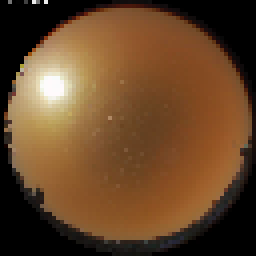
\includegraphics[width=1.2cm]{figures/arch/hist_t0.png}};
  \foreach \k/\o in {2/0.16, 1/0.08, 0/0}
    \node[pic] at (2.35+\o,\yI+\o) {\includegraphics[width=1.2cm]{figures/arch/noise_\k.png}};
  \node[align=center, anchor=north] at (0.75,\yI-0.62) {history\\$\mathbf{I}_{t-14:t}$};
  \node[align=center, anchor=north] at (2.35,\yI-0.62) {noisy future\\$\mathbf{x}^{I}_{\tau}$};
  \begin{axis}[pvaxis, at={(0.15cm,-0.55cm)}, width=2.96cm, ymin=-3, ymax=3, xtick=\empty, ytick=\empty]
    \addplot[pvline, mark=*, mark size=0.7pt] table[x=min, y=v, col sep=comma] {figures/arch/pv_in_hist.csv};
    \addplot[black!55, only marks, mark=*, mark size=0.7pt] table[x=min, y=v, col sep=comma]
      {figures/arch/pv_in_noise.csv};
    \draw[densely dotted, black!50] (1,-3) -- (1,3);
  \end{axis}
  \node[anchor=south] at (0.89,0.58) {history};
  \node[anchor=south] at (2.37,0.58) {noisy future $\mathbf{x}^{p}_{\tau}$};
  \node[rotate=90, font=\footnotesize] at (-0.2,\yI) {Sky images};
  \node[rotate=90, font=\footnotesize] at (-0.2,\yP) {PV power};
  % ======== sky-image U-Net (block height ~ spatial resolution) ========
  \node[iblk, minimum height=12mm]  (e1) at (4.45,\yI)  {$64^2$\\16};
  \node[iblk, minimum height=9mm]   (e2) at (5.70,\yI)  {$32^2$\\32};
  \node[iblk, minimum height=7.5mm] (e3) at (6.95,\yI)  {$16^2$\\64};
  \node[iblk, minimum height=6mm]   (e4) at (8.20,\yI)  {$8^2$\\128};
  \node[iblk, minimum height=7.5mm] (d3) at (9.45,\yI)  {$16^2$\\64};
  \node[iblk, minimum height=9mm]   (d2) at (10.70,\yI) {$32^2$\\32};
  \node[iblk, minimum height=12mm]  (d1) at (11.95,\yI) {$64^2$\\16};
  % ======== PV U-Net (sequence length 16 at every level) ========
  \node[pblk] (p1) at (4.45,\yP)  {16};
  \node[pblk] (p2) at (5.70,\yP)  {32};
  \node[pblk] (p3) at (6.95,\yP)  {64};
  \node[pblk] (p4) at (8.20,\yP)  {128};
  \node[pblk] (q3) at (9.45,\yP)  {64};
  \node[pblk] (q2) at (10.70,\yP) {32};
  \node[pblk] (q1) at (11.95,\yP) {16};
  \draw[->] (3.2,\yI) -- (e1);
  \draw[->] (3.11,\yP) -- (p1);
  \draw[->] (e1) -- node[op]{$\downarrow2$} (e2);
  \draw[->] (e2) -- node[op]{$\downarrow2$} (e3);
  \draw[->] (e3) -- node[op]{$\downarrow2$} (e4);
  \draw[->] (e4) -- node[op]{$\uparrow2$} (d3);
  \draw[->] (d3) -- node[op]{$\uparrow2$} (d2);
  \draw[->] (d2) -- node[op]{$\uparrow2$} (d1);
  \foreach \a/\b in {p1/p2, p2/p3, p3/p4, p4/q3, q3/q2, q2/q1} \draw[->] (\a) -- (\b);
  \draw[skip] (e3.north) -- ++(0,0.35) -| (d3.north);
  \draw[skip] (e2.north) -- ++(0,0.40) -| (d2.north);
  \draw[skip] (e1.north) -- ++(0,0.42) -| (d1.north);
  \draw[skip] (p3.south) -- ++(0,-0.20) -| (q3.south);
  \draw[skip] (p2.south) -- ++(0,-0.40) -| (q2.south);
  \draw[skip] (p1.south) -- ++(0,-0.60) -| (q1.south);
  % ======== RS-PV-MMA coupling at levels 2-4 ========
  \foreach \k/\w/\x in {2/1/5.70, 3/4/6.95, 4/8/8.20} {
    \node[mma] (m\k) at (\x,\yM) {MMA\\$w{=}\w$};
    \draw[<->] (e\k.south) -- (m\k.north);
    \draw[<->] (m\k.south) -- (p\k.north);
  }
  % ======== diffusion-step embedding ========
  \node (tau) at (0.2,\yM) {$\tau$};
  \node[draw, minimum height=6mm, align=center, inner sep=1.5pt] (temb) at (1.55,\yM) {sinusoidal\\emb.\ + MLP};
  \node[draw, circle, inner sep=0.6pt] (et) at (4.45,\yM) {$\mathbf{e}_\tau$};
  \draw[->] (tau) -- (temb);
  \draw[->] (temb) -- (et);
  \draw[->] (et) -- (e1.south);
  \draw[->] (et) -- (p1.north);
  \node[anchor=west, align=left, black!70] at (4.5,2.35) {every\\block};
  % ======== DDIM update and sampling loop ========
  \draw[fill=black!6] (12.75,\yP-0.4) rectangle (13.35,\yI+0.65);
  \node[rotate=90, align=center] at (13.05,{(\yI+\yP+0.25)/2}) {DDIM update ($\eta{=}0$)\\$\mathbf{x}_{\tau_i}\rightarrow\mathbf{x}_{\tau_{i-1}}$};
  \draw[->] (d1) -- node[op]{$\hat{\boldsymbol\epsilon}^{I}$} (12.75,\yI);
  \draw[->] (q1) -- node[op]{$\hat{\boldsymbol\epsilon}^{p}$} (12.75,\yP);
  \draw[loop] (13.05,\yI+0.65) -- (13.05,\yI+1.4) -- node[above]{$\mathbf{x}_{\tau_{i-1}}$ is fed back;
    $S{=}15$ steps from $\mathbf{x}_T\sim\mathcal{N}(\mathbf{0},\mathbf{I})$ to $\hat{\mathbf{x}}_0$} (2.51,\yI+1.4)
    -- (2.51,\yI+0.76);
  \draw[loop] (13.05,\yP-0.4) -- (13.05,\yP-1.2) -- (2.37,\yP-1.2) -- (2.37,\yP-0.55);
  % ======== outputs: DDIM-generated frames (member 1) vs. observed, and the PV ensemble ========
  \draw[->] (13.35,\yI) -- (13.8,\yI);
  \draw[->] (13.35,\yP) -- (13.8,\yP);
  \foreach \k/\x/\l in {02/14.3/2, 08/15.42/8, 16/16.54/16} {
    \node[pic] at (\x,\yI) {\includegraphics[width=1cm]{figures/arch/gen_\k.png}};
    \node[pic] at (\x,\yI-1.3) {\includegraphics[width=1cm]{figures/arch/obs_\k.png}};
    \node[anchor=north] at (\x,\yI-1.82) {$+\l$ min};
  }
  \node[anchor=south] at (15.42,\yI+0.52) {generated $\hat{\mathbf{I}}$ (member 1)};
  \node at (15.42,\yI-0.65) {observed $\mathbf{I}$};
  \begin{axis}[pvaxis, at={(13.8cm,-0.55cm)}, width=3.24cm, ymin=2.5, ymax=7.5, xtick={-14,0,16},
      ytick={3,5,7}, yticklabel pos=right]
    \addplot[fill=pvline!28, draw=none] table[x=min, y=kw, col sep=comma] {figures/arch/pv_band.csv};
    \addplot[black, mark=*, mark size=0.6pt] table[x=min, y=kw, col sep=comma] {figures/arch/pv_hist.csv};
    \addplot[pvline, line width=0.9pt] table[x=min, y=med, col sep=comma] {figures/arch/pv_fut.csv};
    \addplot[black, only marks, mark=o, mark size=0.9pt] table[x=min, y=obs, col sep=comma]
      {figures/arch/pv_fut.csv};
    \draw[densely dotted, black!50] (0,2.5) -- (0,7.5);
  \end{axis}
  \node[anchor=south] at (15.42,0.58) {PV ensemble, $M{=}30$ (kW)};
  % ======== legend ========
  \begin{scope}[shift={(0.9,-1.85)}]
    \draw[draw=imgline, fill=imgfill] (0,-0.1) rectangle ++(0.3,0.2);
    \node[right] at (0.3,0) {sky-image block};
    \draw[draw=pvline, fill=pvfill] (2.3,-0.1) rectangle ++(0.3,0.2);
    \node[right] at (2.6,0) {PV block};
    \draw[fill=black!6] (4.0,-0.1) rectangle ++(0.3,0.2);
    \node[right] at (4.3,0) {MMA: RS-PV-MMA cross-attention};
    \draw[skip] (8.6,0) -- ++(0.5,0);
    \node[right] at (9.1,0) {skip (concat.)};
    \node[right] at (11.0,0) {$\downarrow2$ / $\uparrow2$: max pool / bilinear up-sampling};
  \end{scope}
\end{tikzpicture}
\caption{Coupled U-Net denoiser and DDIM sampling (compact form of PV-MM-Diffusion~\cite{huang2026pvmm}) on a real
test window (2019-07-14 08:12). Inputs: 8 history frames and PV readings followed by 8 future frames that start as
noise (PV in normalized scale). Image blocks are labelled with spatial size and channels, PV blocks with channels;
RS-PV-MMA with temporal window $w$ couples the branches at levels 2--4, and $\mathbf{e}_\tau$ enters every block.
Outputs after 15 DDIM steps: generated frames of the first member vs.\ observed ones, and the 30-member PV forecast
(band: 5--95\%; line: median; dots/circles: observed history/future).}
\label{fig:arch}
\end{figure*}

\subsection{DDIM Sampling}
At inference the future block starts from Gaussian noise and is denoised with DDIM~\cite{song2021ddim} on an evenly
spaced sub-sequence $\tau_S>\dots>\tau_0=0$ of the training steps. With
$\hat{\mathbf{x}}_0=(\mathbf{x}_{\tau_i}-\sqrt{1-\bar\alpha_{\tau_i}}\,\epsilon_\theta)/\sqrt{\bar\alpha_{\tau_i}}$
and $\eta=0$, each update is deterministic,
\begin{equation}
  \mathbf{x}_{\tau_{i-1}}=\sqrt{\bar\alpha_{\tau_{i-1}}}\,\hat{\mathbf{x}}_0
  +\sqrt{1-\bar\alpha_{\tau_{i-1}}}\;\epsilon_\theta(\mathbf{x}_{\tau_i},\tau_i),
\end{equation}
so ensemble members differ only through their initial noise. We use $S=15$ steps and clip sampled PV to
$[0,P_{\max}]$. DDIM with $\eta=0$ is the first-order solver of the probability-flow ODE that DPM-Solver++ integrates
at higher order; as other factors also differ (Table~\ref{tab:diff}), we do not isolate the solver's effect.

%=====================================================================
\section{Experimental Setup}
%=====================================================================
\textit{Data and split.} SKIPP'D~\cite{nie2023skippd} pairs $64\times64$ sky images at 1-minute resolution with the
power of a 30~kW array at Stanford University (349{,}372 training and 14{,}003 test records). Windows of 16 frames at a
2-minute cadence are taken within a day, skipping logging gaps. A seeded 10\% of \emph{calendar days} is held out for
validation to avoid leakage between overlapping windows. The test set has 1{,}340 windows over 20 clear, partly cloudy
and overcast days, 1{,}115 of them daytime (mean output above 15\% of capacity). The reference instead tests on five
multi-cloud days of the SkyGPT partition~\cite{nie2024skygpt}, so only relative improvements are comparable.

\textit{Baselines.} \emph{Smart persistence (SPM)} holds the clear-sky index $k=p_t/p^{\mathrm{clr}}_t$ constant,
$\hat p_{t+h}=k\,p^{\mathrm{clr}}_{t+h}$~\cite{sun2019sunset}, with $p^{\mathrm{clr}}$ the Ineichen--Perez clear-sky
irradiance from pvlib~\cite{holmgren2018pvlib} scaled to 30~kW. The \emph{two-stage pipeline} stands in for
SkyGPT$\rightarrow$U-Net: a 3-D CNN video predictor followed by a CNN that regresses PV from future frames and past
PV, each trained with a squared-error loss and fed Stage~1's predictions at test time. The \emph{PV-only ablation}
samples the trained joint model in mode~(iii) with all past images replaced by placeholders.

\textit{Implementation.} Models are implemented in TensorFlow 2.14 and trained with Adam~\cite{kingma2015adam}
(learning rate $2\times10^{-4}$, batch size 8) on one NVIDIA RTX~3070
(8~GB), which also runs all inference. Early stopping monitors the validation diffusion loss (patience 10), and the
best checkpoint is tested. Seeds are fixed to 42 and the ensemble size is $M=30$.

\begin{figure*}[t]
\centering
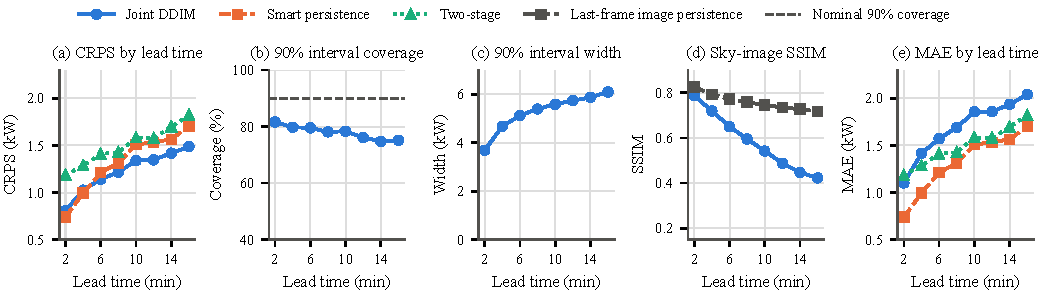
\includegraphics[width=0.92\textwidth]{figures/lead_diagnostics.pdf}
\caption{Performance by lead time on the 1{,}340 test windows. (a) CRPS of the DDIM ensemble, smart persistence and
the two-stage pipeline (equal to MAE for the deterministic baselines). (b) Coverage and (c) mean width of the DDIM
90\% interval. (d) SSIM of DDIM-generated frames (first member) and last-frame persistence against the observed
future frames. (e) MAE of the DDIM ensemble median, smart persistence and the two-stage pipeline.}
\label{fig:lead}
\end{figure*}

\textit{Metrics.} For an observation $y$ and ensemble $\{\hat y^{(m)}\}_{m=1}^M$, the primary metric is the empirical
CRPS~\cite{lauret2019verification},
\begin{equation}
  \mathrm{CRPS}=\frac1M\sum_{m}\big|\hat y^{(m)}-y\big|-\frac{1}{2M^2}\sum_{m,m'}\big|\hat y^{(m)}-\hat y^{(m')}\big|,
\end{equation}
averaged over windows and lead times; for $M=1$ it equals the mean absolute error (MAE). Skill is
$1-\mathrm{CRPS}/\mathrm{CRPS}_{\mathrm{SPM}}$. The central 90\% interval (5th--95th ensemble percentiles) is scored
by the Winkler score (WS$_{90}$)~\cite{vandermeer2018review}, coverage and width. Point accuracy of the ensemble median
and mean is given by MAE, RMSE, mean bias error (MBE) and $R^2$. Generated frames are compared with observed ones by
SSIM and the cosine similarity of VGG-16 features~\cite{simonyan2015vgg} (VGG-CS), as is standard in video
prediction~\cite{lee2018savp}, with last-frame persistence as reference.

%=====================================================================
\section{Results}
%=====================================================================
\textit{Probabilistic accuracy.} Table~\ref{tab:main} shows that the joint DDIM ensemble has the lowest CRPS,
\SI{\ddimcrps}{kW}, 7.5\% better than smart persistence and 18.4\% better than the two-stage pipeline. The latter is
13.4\% worse than persistence, because errors in its predicted video propagate to a PV regressor trained on true
frames; the joint model denoises both outputs together and avoids this mismatch. The 18.4\% gain matches the 18\%
reported for PV-MM-Diffusion~\cite{huang2026pvmm} despite a 4$\times$ shorter sampler, a lighter backbone and all-sky
test days, though with a different decoupled baseline. Our lower absolute CRPS mainly reflects the easier all-sky
test set. Withholding the sky images raises the CRPS by 70\% to \SI{2.072}{kW} and doubles the Winkler score, so the
images carry most of the predictive information.

\begin{table}[t]
\centering
\caption{Probabilistic Accuracy on the SKIPP'D Test Set (1{,}340 Windows, 2--16 min). Skill vs.\ Smart Persistence; Nominal Coverage 90\%.}
\label{tab:main}
\footnotesize
\setlength{\tabcolsep}{3pt}
\begin{tabular}{@{}lcccc@{}}
\toprule
Method & CRPS (kW) & Skill & WS$_{90}$ (kW) & Cov.$_{90}$ \\
\midrule
Smart persistence$^{\dagger}$ & 1.321 & \phantom{$-$}0.0\% & -- & -- \\
Two-stage pipeline$^{\dagger}$ & 1.498 & $-$13.4\% & -- & -- \\
Joint DDIM, PV-only input & 2.072 & $-$56.8\% & 20.61 & -- \\
\textbf{Joint DDIM, SI+PV input} & \textbf{1.222} & \textbf{+7.5\%} & \textbf{10.50} & 77.9\% \\
\bottomrule
\end{tabular}\\[2pt]
{\scriptsize $^{\dagger}$Deterministic: CRPS reduces to MAE; interval scores are undefined.}
\end{table}

\begin{table}[t]
\centering
\caption{Point-Forecast Accuracy and CRPS (All 1{,}340 Windows; Daytime MAE in Brackets)}
\label{tab:point}
\footnotesize
\setlength{\tabcolsep}{2.5pt}
\begin{tabular}{@{}lccccc@{}}
\toprule
Method & CRPS$^{\ast}$ & MAE & RMSE & MBE & $R^2$ \\
 & (kW) & (kW) & (kW) & (kW) & \\
\midrule
Smart persistence & 1.321 & \textbf{1.321} [\textbf{1.481}] & 3.087 & \textbf{$-$0.035} & 0.824 \\
Two-stage & 1.498 & 1.498 [1.608] & \textbf{2.838} & 0.172 & \textbf{0.851} \\
DDIM median & \multirow{2}{*}{\textbf{1.222}} & 1.684 [1.899] & 2.960 & $-$0.763 & 0.838 \\
DDIM mean & & 1.823 [2.046] & 2.956 & $-$0.837 & 0.839 \\
\bottomrule
\end{tabular}\\[2pt]
{\scriptsize $^{\ast}$Of the full 30-member DDIM ensemble; equal to MAE for the deterministic baselines.}
\end{table}

\begin{figure}[!t]
\centering
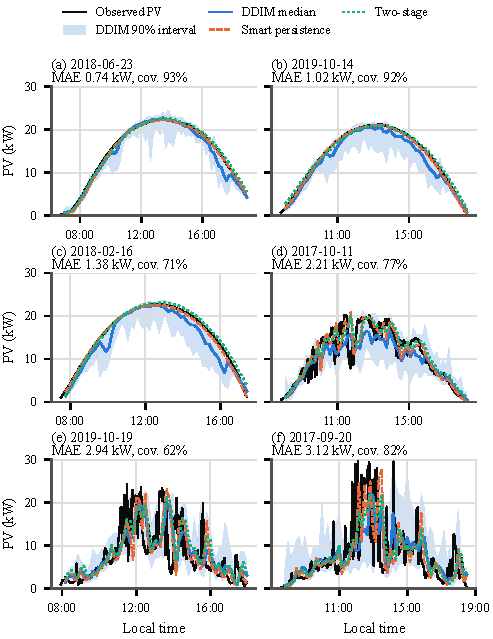
\includegraphics[width=\columnwidth]{figures/daily_timeseries.pdf}
\caption{16-minute-ahead forecasts on six test days at evenly spaced ranks of PV variability, from (a) least to (f)
most variable. Band: DDIM 90\% interval (30 members); panel titles give the day's DDIM median MAE and coverage.}
\label{fig:days}
\end{figure}

\begin{figure}[!t]
\centering
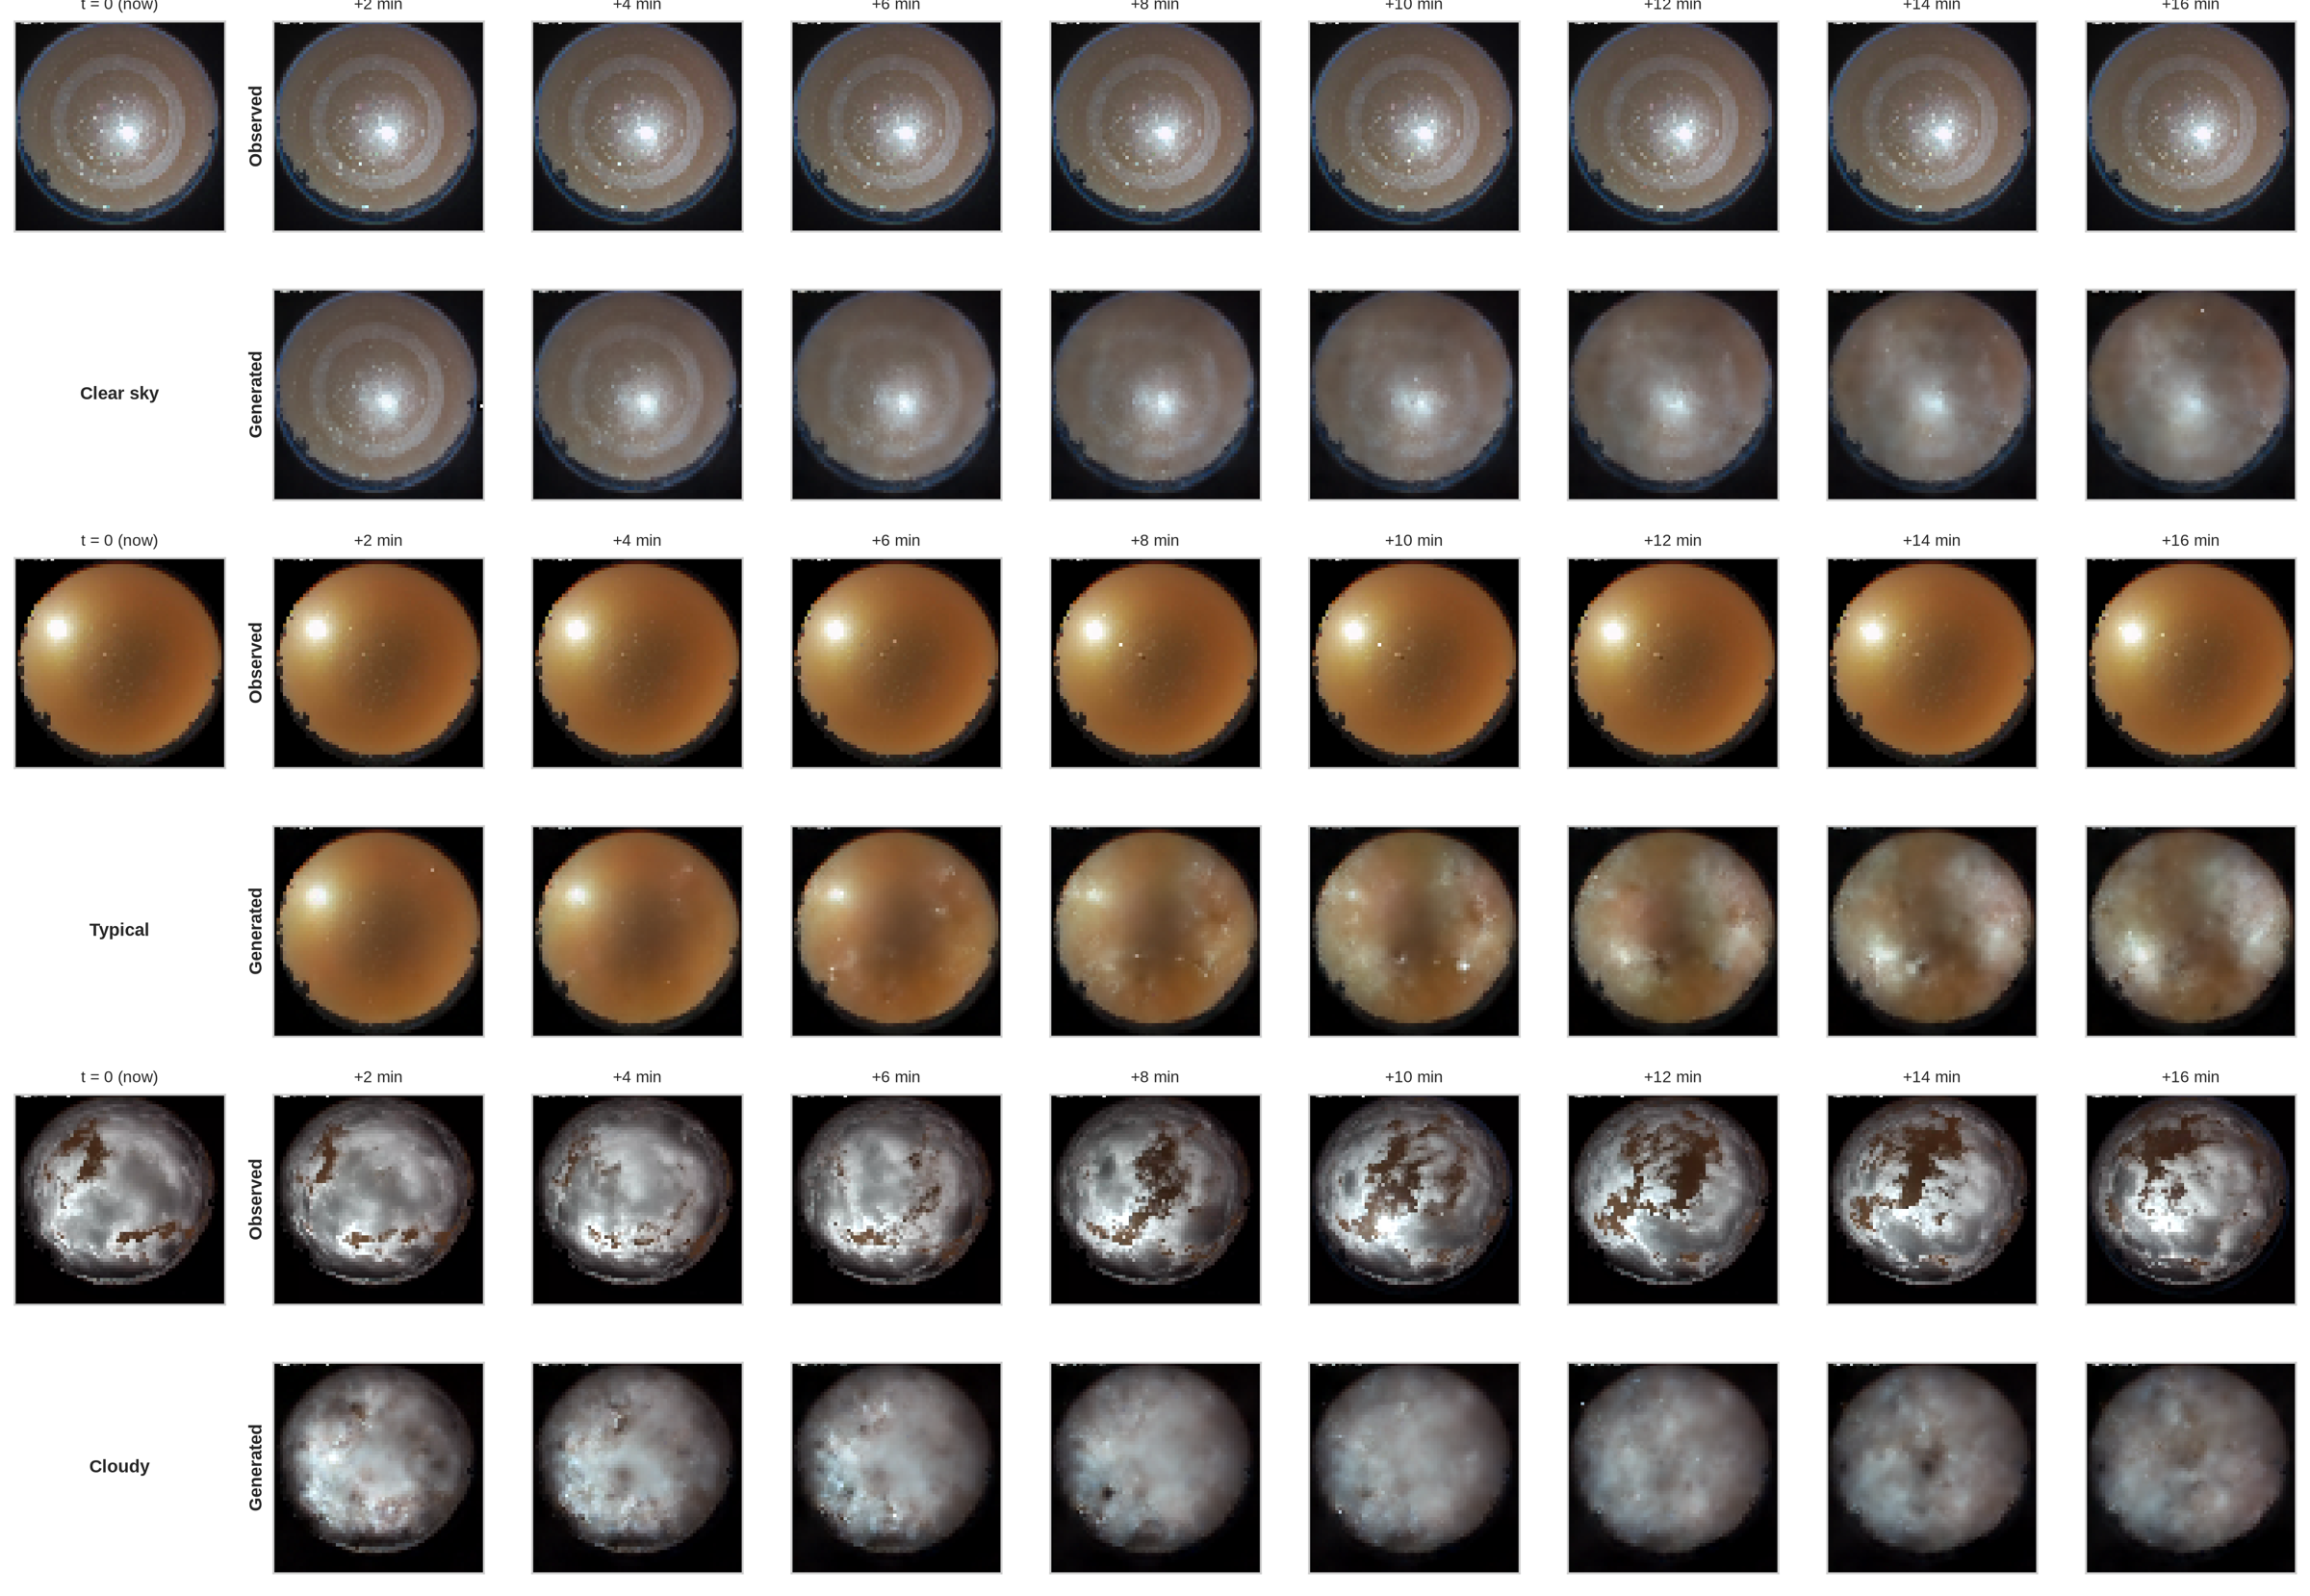
\includegraphics[width=0.88\columnwidth]{figures/sky_images.png}
\caption{Observed (upper row of each pair) and DDIM-generated (lower row, first member) sky images for the daytime
test windows with the lowest, median and highest PV variability. The first column is the last observed frame.}
\label{fig:sky}
\end{figure}

\textit{Calibration.} The 90\% intervals cover 77.9\% of observations, so the ensemble is under-dispersed.
Fig.~\ref{fig:lead}(b,c) shows that coverage falls from 81.6\% at +2~min to 75.1\% at +16~min while the mean width
grows from 3.69 to \SI{6.10}{kW}: the spread increases with lead time, but not as fast as the errors. With $\eta=0$
the only source of diversity is the initial noise, and 15 steps pass quickly through the high-noise regime, which is a
plausible cause.

\textit{Point accuracy.} As a point forecast the picture reverses (Table~\ref{tab:point}). The DDIM median has the
highest MAE (\SI{1.684}{} vs.\ \SI{1.321}{kW} for persistence) but a lower RMSE than persistence and a higher $R^2$,
i.e., many moderate errors but fewer large ones: its 99th-percentile absolute error is \SI{12.68}{kW} against
\SI{14.72}{kW} for persistence, which fails at ramps that the image-conditioned model partly anticipates. The DDIM
forecasts are biased low (MBE $-0.76$~kW for the median), which is most visible as afternoon dips on clear days
(Fig.~\ref{fig:days}(a)--(c)); on the most variable day (f), the 90\% band widens during the midday ramps while
persistence reproduces each ramp one lead time late. Persistence is best at +2~min, and the relative MAE gap narrows from 49\% at +2~min to 20\% at +16~min
(Fig.~\ref{fig:lead}(e)). The CRPS rewards an ensemble whose spread covers the observation even when its centre is
off, so the model's advantage lies in its distribution, not its central estimate.

\textit{Generated images and cost.} The generated frames reach a VGG-CS of 0.862. They preserve the sun position and
large-scale cloud layout for the first minutes and then blur and lose fine structure, and on the clear-sky example
they gradually add spurious haze (Fig.~\ref{fig:sky}); SSIM falls from 0.787 at +2~min to
0.423 at +16~min, whereas last-frame persistence falls only from 0.826 to 0.717 (Fig.~\ref{fig:lead}(d)). At this
capacity the image branch does not model cloud advection faithfully beyond a few minutes. Sampling takes
\SI{155.5}{ms} per window per member on the RTX~3070 (\SI{4.7}{s} for 30 members) and grows almost linearly with the
step count (56 and 249~ms at 10 and 60 steps). The reference needs \SI{45.39}{s} for 10 members on an
RTX~3090~\cite{huang2026pvmm}, about 29 times our per-member cost, owing to both sampler and network size.

%=====================================================================
\section{Discussion and Limitations}
\label{sec:disc}
%=====================================================================
Joint diffusion gives the best probabilistic score and clearly beats a decoupled video-then-PV pipeline, supporting
the central claim of~\cite{huang2026pvmm} on all-sky days with a 15-step sampler on one GPU. It is, however,
under-dispersed, biased low and weaker than persistence as a point forecaster. Remedies include stochastic sampling
($\eta>0$) and larger ensembles, post-hoc recalibration, predicting the residual to smart persistence, and larger
backbones or latent diffusion~\cite{gao2023prediff}. Whether the weaknesses stem from our reductions cannot be
decided here; testing on the SkyGPT partition, sampling one model with both solvers and restoring patch-level
cross-attention would separate the factors. The study covers one site, one horizon, 20 test days and one training run.

%=====================================================================
\section{Conclusion}
%=====================================================================
We evaluated a compact single-GPU re-implementation of PV-MM-Diffusion sampled with 15-step DDIM. On 1{,}340 all-sky
SKIPP'D test windows, the 30-member ensemble achieves a CRPS of \SI{1.222}{kW}, improving on smart persistence by
7.5\% and on a two-stage pipeline by 18.4\%, at \SI{155}{ms} per member, but it is under-dispersed (77.9\% coverage
of 90\% intervals), biased low and weaker than persistence as a point forecaster. Closing these calibration and bias
gaps is the clearest route to operational use.

\bibliographystyle{IEEEtran}
\bibliography{refs}

\end{document}
